\section{Exploratory support-matched spectral extension}
\label{sec:m2-extension}

The earlier results motivate a separate investigation of the representation and
fusion used by MIRA-CSI, rather than an assumption that a larger neural model
must improve transfer. We evaluate five explicitly defined arms, A--E, in a
frozen 75-fit execution. The research direction was developed after historical
target outcomes had been observed. Although all five arms and the primary
comparison were fixed before this execution's test evaluation, the extension
is exploratory, not a fresh preregistered confirmation. E was a declared
feature-only comparator; its prominence below follows its observed result and
must not be retrospectively presented as the original main hypothesis.

\subsection*{Prior work and scope of the construction}
Covariance-based CSI features predate this extension. PADS uses eigenvalues of
covariance matrices from normalized CSI amplitude and phase for binary motion
detection~\cite{m2pads}. Covariance-normalized temporal variation also has a
long history: slow feature analysis (SFA) minimizes temporal change under
variance/decorrelation constraints~\cite{m2sfa}, while second-order blind
identification (SOBI) uses joint diagonalization of lagged covariance matrices
for source separation~\cite{m2sobi}. The present classifier is neither a new
invention of covariance eigenspectra nor an implementation of SFA or SOBI.
It combines an explicitly defined observed-endpoint normalization with a
fixed cell/lag grid and compares its use in feature-only and hybrid models.
PADS's binary task and acquisition protocol are not a matched seven-class
baseline, so its reported detection rates are not compared with our accuracy.

Missingness indicators and elapsed-time information are established model
inputs~\cite{che2018}. Mask-aware renormalized filtering likewise has prior
art~\cite{m2partial}; the CNN here does not implement the partial-convolution
mask-update rule. Our distance is the normalized distance to the nearest
observed position in either direction, making the implementation offline.
We claim neither causal streaming nor a new principle of missing-data handling.

\subsection*{Data representation and source-only roles}
We retain the existing immutable selection of 1,260 genuine recordings from
the public Alsaify et al. dataset~\cite{multienvdata}: 30 participants, ten in each
of three environments, seven selected activity segments and six selected
trials per subject/segment. This subset is not the entire source dataset.
The seven labels are sitting, falling from sitting, lying, standing, walking
between transmitter and receiver, sitting down, and picking up an object.

This extension uses a fixed \emph{log-mean scaled power} representation, which
differs from the earlier mean-log-amplitude representation. Let
$H^{\mathrm{sc}}_{r,k}(j)$ be the previously scaled complex CSI for receive
antenna $r$, exported-subcarrier index $k$ and valid packet index $j$.
For consecutive groups $\mathcal G_b$ of five exported subcarriers, the fixed
per-record conversion is
\begin{equation}
 q_{r,b}(j)=10\log_{10}\!\left[
 \max\!\left\{\frac{1}{5}\sum_{k\in\mathcal G_b}
 |H^{\mathrm{sc}}_{r,k}(j)|^2,10^{-24}\right\}\right].
 \label{eq:m2-power}
\end{equation}
Three receiving antennas and six groups yield 18 streams, each linearly
resampled to 500 equally spaced valid-packet-index positions. These are dB
values of dimensionless scaled channel power, not calibrated dBm, body heat,
or a physical image. Original recording duration and irregular packet timing
are not preserved. The conversion is recordwise and unfitted; no pooled target
statistics are used. Changing this representation is a preprocessing choice,
not evidence of a new sensing capability.

For each excluded environment $e\in\{1,2,3\}$, the other two environments
provide 504 source-training recordings from 12 participants, 168 validation
recordings from four other participants, and 168 familiar-environment test
recordings from another four participants. All 420 recordings from the ten
participants in $e$ form the held-environment test. Participants are disjoint
between roles within each fold. Since each environment has a different
participant cohort, this evaluates joint environment--cohort transfer; it
cannot identify a causal room effect. Familiar-test participants can recur in
other outer folds, so familiar scores are reported per fold, not treated as
independent new cohorts in a pooled confidence calculation.

Per-band population means and standard deviations are fitted only over source
training files and positions. Standard deviations have a $10^{-6}$ lower
bound. The temporal path subtracts/divides those statistics only at observed
entries, then assigns exact zero to hidden entries. The fixed spectral branch
uses the raw observed values of the processed power tensor. Consequently its
no-hidden-value property concerns simulated loss \emph{after} the fixed
packet-index conversion, not missing raw acquisition packets before
resampling or power scaling.

\subsection*{Matched endpoint statistics and numerical implementation}
Write $x_t\in\mathbb R^{18}$ for one processed recording and
$m_t\in\{0,1\}$ for its shared temporal observation mask. For a cell
$B=[a,b)$ and lag $\ell$, retain the original index pairs
\begin{equation}
 \begin{aligned}
 \mathcal P_{B,\ell}&=
 \{t:a\leq t<b-\ell,\ m_t=m_{t+\ell}=1\},\\
 n&=|\mathcal P_{B,\ell}|.
 \end{aligned}
 \label{eq:m2-pairs}
\end{equation}
Only the two endpoints need be observed. Missing interior positions do not
remove a pair, and remaining observations are never compressed together.
For $a_i=x_{t_i}$ and $b_i=x_{t_i+\ell}$, define
\begin{align}
 \mu_P&=\frac{1}{2n}\sum_{i=1}^{n}(a_i+b_i),\label{eq:m2-mean}\\
 N&=\frac{1}{2n}\sum_{i=1}^{n}(b_i-a_i)(b_i-a_i)^\top,\label{eq:m2-N}\\
 D_P&=\frac{1}{2n}\sum_{i=1}^{n}
 \big[(a_i-\mu_P)(a_i-\mu_P)^\top\nonumber\\[-2pt]
 &\hspace{28mm}+(b_i-\mu_P)(b_i-\mu_P)^\top\big].\label{eq:m2-D}
\end{align}
Here $N$ is an \emph{uncentered increment second moment}, with the intentional
factor $1/2$; it is not the covariance of mean-subtracted increments. Both
moments use the same multiset of observed pair endpoints. A position can
occur in more than one pair, so endpoint multiplicities enter $D_P$.

With $u_i=a_i-\mu_P$ and $v_i=b_i-\mu_P$,
\begin{equation}
 2D_P-N=\frac{1}{2n}\sum_i(u_i+v_i)(u_i+v_i)^\top\succeq0.
 \label{eq:m2-bound}
\end{equation}
Thus $0\preceq N\preceq2D_P$. Since
$\ker(D_P)\subseteq\ker(N)$, the finite generalized spectrum on the full
effective covariance support lies in $[0,2]$. This algebraic property defines
the construction; it is not an empirical guarantee of correct classification.

The implementation computes symmetric float64 moments and diagonalizes $D_P$.
If $D_P=U\operatorname{diag}(d_i)U^\top$, retain
$I=\{i:d_i>10^{-8}d_{\max}\}$. It forms
\begin{equation}
 W=\operatorname{diag}(d_i^{-1/2})_{i\in I}U_I^\top,\qquad
 \lambda=\operatorname{eig}(WNW^\top).
 \label{eq:m2-whiten}
\end{equation}
The matrix is symmetrized before eigendecomposition. A violations tolerance
of $10^{-4}$ is used: violations beyond the allowed negative or matched upper
bound raise an error, while small allowed violations are clipped. The retained
eigenvalues are sorted and transformed as
\begin{equation}
 z_i=\log\big(0.999\lambda_i+0.001\big).
 \label{eq:m2-log}
\end{equation}
Eighteen entries are reserved per cell/lag; unused entries are zero, equivalent
to the neutral transformed value at $\lambda=1$. With fewer than 36 endpoint
pairs or zero effective rank, the block is neutral and its validity flag is
zero. No difficult recording is dropped. A valid block's flag is one; the
pair fraction $n/(b-a-\ell)$ is also retained. Padding does not uniquely
identify rank, and neither flag nor pair fraction is a physical confidence.

The cells are $[0,500)$, $[0,250)$ and $[250,500)$, with lags
$\{1,2,4,8,16,32\}$. Across 18 cell/lag combinations, concatenating
$18\times18=324$ spectral entries, 18 validity flags and 18 pair fractions
gives 360 float32 classifier inputs. Fully observed per-record features are
cached; a corrupted recording's features are recomputed under its actual mask.
No clean hidden values are supplied through the cache.

For the all-observed comparator B, $N$ is unchanged but $D_P$ is replaced by
\begin{equation}
 \begin{aligned}
 D_O&=\frac{1}{M}\sum_{t\in O_B}(x_t-\mu_O)(x_t-\mu_O)^\top,\\
 O_B&=\{t\in B:m_t=1\}.
 \end{aligned}
 \label{eq:m2-B}
\end{equation}
Here $M=|O_B|$ and $\mu_O$ is the uniform observed-cell mean. B's spectrum
need not be bounded above by 2 and is not clipped at 2. This comparator
changes endpoint weighting, centering, and potentially included positions.
It differs from A even when every position is observed: for non-cyclic lag-1
pairs, endpoint multiplicities are $[1,2,\ldots,2,1]$ rather than uniform.
Therefore A--B does not isolate an effect present only under missingness.

C replaces the full-matrix quotients by matched per-channel diagonal ratios
$N_{jj}/(D_P)_{jj}$ in fixed channel order. Positive diagonal variance is
required; zero-variance channels receive neutral ratio 1, and an entirely
zero-variance block is invalid. Unlike A/B, C has no relative full-matrix
rank threshold or sorted-spectrum padding. It is a useful simpler alternative,
not a pure deletion of off-diagonal entries with every other rule unchanged.

\paragraph{Scope of invariance.}
For the same mask, cell and lag, an ideal fixed nonsingular affine channel
map $x'_t=Gx_t+c$ yields $N'=GNG^\top$ and $D'_P=GD_PG^\top$.
The untruncated generalized spectrum on the full effective support is
unchanged. \emph{B shares this ideal congruence invariance}, because its
observed-cell covariance obeys the same transformation law. Matching supplies
the common endpoint reference and the $[0,2]$ bound, not the origin of
invariance absent from B. This nuisance model is not a physical law for
arbitrary room, participant, multipath or antenna changes.

The implemented threshold can change the retained subspace even if the
retained rank does not change. For example, use three active directions with
$D=\operatorname{diag}(1,9\times10^{-9},2\times10^{-8})$ and
$N=D\operatorname{diag}(0.2,0.8,1.5)$. Under
$G=\operatorname{diag}(1,2,0.5)$, whose condition number is 4, the relative
threshold retains rank 2 before and after transformation, but the retained
spectra change from $[0.2,1.5]$ to $[0.2,0.8]$. Exact null directions can pad
this example to 18 dimensions. Stable retained subspaces and adequate numerical
conditioning, not merely unchanged rank, are required for a numerical
invariance approximation. The threshold, clipping, log floor and padding
qualify the implementation; the hybrid CNN is not generally affine invariant.

\subsection*{Arms, training and frozen evaluation}
Table~\ref{tab:m2-arms} defines all five arms. For A--D, the temporal encoder
receives 18 normalized channels, the mask, and the symmetric nearest-observation
distance divided by 500. Three Conv1d blocks use output widths 32, 64, 128;
kernels 7, 5, 3; stride 2 and same-style padding; each is followed by
eight-group GroupNorm and GELU. Final temporal pooling weights are adaptive
averages of the mask, lower bounded by 0.05. GroupNorm mixes temporal positions;
these weights are a heuristic, not exact local receptive-field support.

For A--C and E, a 360--64--32 MLP with GELU after each linear layer encodes
the fixed features. A--C concatenate this vector with the 128-dimensional
temporal representation; D retains only the temporal vector; E retains only
the feature vector. Dropout 0.2 precedes a seven-logit linear classifier.
The trainable counts are 66,279 for A/B/C, 40,871 for D and 25,415 for E.
Removing a path also changes capacity, so D/E are not parameter-matched
interventions that identify a unique cause.

All arms use the settings in Table~\ref{tab:m2-protocol}: AdamW with learning
rate $10^{-3}$ and weight decay $10^{-4}$, cross-entropy, batch size 64,
gradient-norm clipping at 5, at most 60 epochs, and stopping after 12 epochs
without a clean source-validation NLL decrease exceeding $10^{-4}$.
The saved best validation-NLL weights are restored. One scalar temperature
$T\in[0.1,10]$ is then fitted on that same clean source validation set by
bounded NLL minimization, following the established temperature-scaling
approach~\cite{guo2017}. Neither fitting step uses familiar or held
recordings to fit or select parameters. The weights and temperature are fixed for all test conditions;
source-only calibration does not guarantee calibration after transfer.

Training retains complete input with probability 0.5. Otherwise it draws
random or contiguous loss uniformly and a missing fraction from
$\{0.1,0.3,0.5\}$ uniformly. Masks are shared across channels and independent
of class labels. A separate NumPy generator resets per training seed, so the
source permutation and augmentation draws match across arms irrespective of
Torch/dropout random-number consumption. There is no choice among imputers:
the implementation uses observed entries with canonical zero-fill and actual-
mask features. Repeating multiple hidden fills would duplicate the same
defined input path rather than measure different repairs.

Training seeds are 20261026--20261030. Five arms, three outer folds and five
seeds give 75 source fits. All final checkpoints, source calibration values,
validation outputs and implementation/input hashes were frozen together and
independently audited before held/familiar model inference. Static per-record
preprocessing and hash reads are distinct from inference or target fitting.
An explicit evaluation-only stage then tested complete input, random 50\%
loss under five fixed mask seeds, and contiguous 50\% loss under the same
five seeds: 11 conditions per fit. Each loss mask removes exactly 250 of the
500 normalized positions, shared across all 18 channels. These are synthetic
post-conversion deletions, not measured wireless outages.

\begin{table*}[t]
\centering
\caption{Frozen comparison arms. All arms use the same source partitions, augmentation draw sequence and optimization settings. A--C have identical nominal trainable parameter counts; D and E change capacity as well as their input paths. The table defines controls, not claims of isolated causal mechanisms.}
\label{tab:m2-arms}
\begingroup\fontsize{9.5}{12}\selectfont
\setlength{\tabcolsep}{5pt}\renewcommand{\arraystretch}{1.13}
\setlength{\extrarowheight}{1.3pt}\setlength{\arrayrulewidth}{0.5pt}\arrayrulecolor{m2border}
\begin{tabularx}{\textwidth}{|llr>{\raggedright\arraybackslash}X|}
\hline\rowcolor{m2head}
\mTwoHead{Arm} & \mTwoHead{Paths} & \mTwoHead{Parameters} & \mTwoHead{Fixed-feature construction} \\
\hline
\rowcolor{m2Afill} A & Temporal + feature MLP & 66,279 & Matched-endpoint generalized lagged-increment spectrum. \\
\hline
\rowcolor{m2Bfill} B & Temporal + feature MLP & 66,279 & Same increment numerator; covariance denominator over all observed cell positions. \\
\hline
\rowcolor{m2Cfill} C & Temporal + feature MLP & 66,279 & Matched per-channel diagonal ratios, kept in channel order. \\
\hline
\rowcolor{m2Dfill} D & Temporal only & 40,871 & No fixed spectral or ratio feature branch. \\
\hline
\rowcolor{m2Efill} E & Feature MLP only & 25,415 & Exactly A's fixed features, without the temporal CNN. \\
\hline
\end{tabularx}
\arrayrulecolor{black}\endgroup
\end{table*}

\begin{table*}[t]
\centering
\caption{Executed extension protocol. This is an exploratory follow-up with historical target outcomes already known; freezing this execution does not make the research direction a fresh preregistered hypothesis.}
\label{tab:m2-protocol}
\begingroup\fontsize{9.5}{12}\selectfont
\setlength{\tabcolsep}{5pt}\renewcommand{\arraystretch}{1.13}
\setlength{\extrarowheight}{1.3pt}\setlength{\arrayrulewidth}{0.5pt}\arrayrulecolor{m2border}
\begin{tabularx}{\textwidth}{|>{\raggedright\arraybackslash}p{.22\textwidth}>{\raggedright\arraybackslash}X|}
\hline\rowcolor{m2head}
\mTwoHead{Item} & \mTwoHead{Executed setting} \\
\hline
\rowcolor{m2Afill} Input & 1,260 selected real recordings; 18 fixed log-mean-power streams by 500 normalized packet positions. \\
\hline
\rowcolor{m2Bfill} Outer-fold roles & 504 training, 168 validation, 168 familiar-test, 420 held-environment recordings. Participants are disjoint within each fold. \\
\hline
\rowcolor{m2Afill} Fixed feature grid & Whole record and two half-record cells; lags 1, 2, 4, 8, 16, 32; at least 36 observed endpoint pairs; 360 features. \\
\hline
\rowcolor{m2Bfill} Numerical choices & Relative covariance eigenvalue threshold $10^{-8}$; log mixture $10^{-3}$; bound violation tolerance $10^{-4}$. \\
\hline
\rowcolor{m2Afill} Training & AdamW, learning rate $10^{-3}$, weight decay $10^{-4}$, batch 64, gradient-norm clip 5, dropout 0.2, at most 60 epochs. \\
\hline
\rowcolor{m2Bfill} Stopping and calibration & Clean source-validation NLL, minimum decrease $10^{-4}$, patience 12; one validation temperature in $[0.1,10]$. \\
\hline
\rowcolor{m2Afill} Augmentation & Probability 0.5 complete; otherwise uniform random/contiguous loss and uniform fraction 0.1/0.3/0.5, same record order and draw sequence for all arms. \\
\hline
\rowcolor{m2Bfill} Repetitions & Training seeds 20261026--20261030; five arms by three folds by five seeds = 75 fits. Five fixed test masks per loss pattern. \\
\hline
\rowcolor{m2Afill} Evaluation & Complete, random 50\%, contiguous 50\%; 11 realizations per fit; all 75 weights and calibration values frozen before held/familiar inference. \\
\hline
\rowcolor{m2Bfill} Primary comparison & A minus B pooled held macro F1 under contiguous 50\% loss. Other arms, input conditions and metrics remain visible. \\
\hline
\end{tabularx}
\arrayrulecolor{black}\endgroup
\end{table*}


The primary contrast remains A minus B held macro F1 under contiguous
50\% loss. For each training-seed/mask-seed cell, we first concatenate the
three disjoint held-fold predictions and score the resulting 1,260 recordings.
For a metric $g$, with $S=5$ training seeds and $K=5$ masks under loss,
\begin{equation}
 \begin{aligned}
 \bar g_s&=\frac1K\sum_{k=1}^{K}g_{s,k},\qquad
 \bar g=\frac1S\sum_{s=1}^{S}\bar g_s,\\
 s_g^2&=\frac1{S-1}\sum_s(\bar g_s-\bar g)^2.
 \end{aligned}
 \label{eq:m2-summary}
\end{equation}
Complete input uses $K=1$. Macro F1 is recomputed from each concatenated
seven-class confusion matrix, rather than averaging fold F1 values.
Per-fold held and familiar metrics are summarized separately by the same
mask-first/seed-second rule. Reported SD is variation over five training seeds
on fixed data, not a participant-population confidence interval. Repeated
masks and fold reuse do not create new independent participants.

For probabilities $p_{ic}$ and class labels $y_i$, NLL is
$-n^{-1}\sum_i\log p_{i,y_i}$ using stable source-temperature log-softmax.
The multiclass Brier score is
$n^{-1}\sum_i\sum_{c=1}^{7}(p_{ic}-\mathbf1[y_i=c])^2$; it is summed over
classes, not divided by seven. Accuracy and unweighted seven-class macro F1
are also retained. Independent audit recomputed metrics directly from saved
logits/probabilities and checked checkpoint, index and protocol bindings.

\subsection*{Results, including negative comparisons}
Table~\ref{tab:m2-pooled} retains all arms and metrics.
A, the main hybrid candidate, reaches only $48.302\pm2.627$\% complete-input
held accuracy and $34.775\pm1.370$\% with contiguous 50\% loss.
B reaches $48.048\pm2.559$\% and $34.187\pm1.598$\%, respectively.
The prespecified primary A--B macro-F1 contrast under contiguous loss is
$+0.543\pm0.654$ percentage points after within-seed mask averaging.
Four training seeds favour A and one favours B. This small, variable difference
does not establish a reliable general benefit from matched normalization.
A post-outcome descriptive difference-of-differences,
$(A-B)_{\mathrm{B50}}-(A-B)_{\mathrm{complete}}$, is
$+0.229\pm0.938$ points, with three positive and two negative seeds; it is
context, not a replacement primary test or a causal estimate.

C gives $44.540\pm1.814$\% complete and $32.311\pm0.740$\% contiguous-loss
held accuracy. D, the temporal-only control in this specific pipeline,
gives $25.222\pm1.609$\% and $21.540\pm2.045$\%. The experiment therefore
does not support an assumption that the hybrid or its additional temporal
path automatically improves cross-cohort transfer.

The declared feature-only arm E performs substantially better in this
execution: $75.175\pm1.005$\% complete accuracy,
$73.822\pm0.942$\% under random 50\% loss and
$60.597\pm1.375$\% under contiguous 50\% loss.
The respective macro F1 values are $74.607\pm1.207$\%,
$73.329\pm1.105$\% and $59.159\pm1.610$\%.
E's NLL increases from $0.773\pm0.018$ to $1.160\pm0.014$, and Brier
from $0.365\pm0.008$ to $0.552\pm0.011$, between complete and contiguous-loss
input. Higher accuracy than the other tested arms does not remove the
substantial loss-related degradation in discrimination or probability quality.

Across held folds E1/E2/E3, E's complete accuracies are
$71.238\pm1.195$\%, $75.381\pm1.289$\% and $78.905\pm1.946$\%;
the contiguous-loss accuracies are $60.486\pm1.239$\%,
$61.086\pm1.407$\% and $60.219\pm2.905$\%.
Although all three fold means exceed 60\% in the latter condition, pooled
seed results for 20261027 and 20261030 are 59.238\% and 59.270\%.
Neither every run nor macro F1 exceeds 60\%.

Familiar-environment scores remain distinct from held scores.
For E, complete familiar accuracy in outer folds E1/E2/E3 is
$75.833\pm1.910$\%, $63.571\pm2.432$\% and $65.833\pm2.511$\%;
contiguous-loss familiar accuracy is $56.024\pm0.661$\%,
$48.524\pm2.825$\% and $55.429\pm2.220$\%.
The familiar cohort is thus not uniformly easier than the held cohort.
This observation is compatible with cohort and activity-trial differences;
it is not evidence of an isolated beneficial room-shift mechanism.
Table~\ref{tab:m2-E} retains E's 18 combinations. Supplementary Tables S1--S6
retain every arm, domain, fold and metric, including unfavourable values.
Figures~\ref{fig:m2-held}--\ref{fig:m2-primary} show all-arm performance,
fold/domain variation and the small paired primary contrast.

\begin{table*}[t]
\centering
\caption{Pooled held-environment results for every prespecified arm. R50 and B50 delete exactly 250 of 500 normalized positions, respectively at random or in one contiguous block. Values are mean $\pm$ sample SD across five training seeds after averaging the five masks within each seed. Accuracy and macro F1 are percentages; NLL and summed multiclass Brier are unitless (lower is better). The same scalar source-validation temperature is retained for every condition.}
\label{tab:m2-pooled}
\begingroup\fontsize{9.5}{12}\selectfont
\setlength{\tabcolsep}{6pt}\renewcommand{\arraystretch}{1.13}
\setlength{\extrarowheight}{1.3pt}\setlength{\arrayrulewidth}{0.5pt}\arrayrulecolor{m2border}
\begin{tabularx}{\textwidth}{|ll*{4}{>{\raggedleft\arraybackslash}X}|}
\hline
\rowcolor{m2head}
\mTwoHead{Arm} & \mTwoHead{Input} & \mTwoHead{Accuracy (\%)} & \mTwoHead{Macro F1 (\%)} & \mTwoHead{NLL} & \mTwoHead{Brier} \\
\hline
\rowcolor{m2Afill}
A & Complete & 48.30\,\(\pm\)\,2.63 & 47.55\,\(\pm\)\,2.93 & 1.395\,\(\pm\)\,0.052 & 0.690\,\(\pm\)\,0.028 \\
\rowcolor{m2Afill}
A & R50 & 49.58\,\(\pm\)\,1.76 & 49.15\,\(\pm\)\,1.99 & 1.327\,\(\pm\)\,0.032 & 0.665\,\(\pm\)\,0.024 \\
\rowcolor{m2Afill}
A & B50 & 34.77\,\(\pm\)\,1.37 & 34.04\,\(\pm\)\,1.38 & 2.127\,\(\pm\)\,0.084 & 0.902\,\(\pm\)\,0.021 \\
\hline
\rowcolor{m2Bfill}
B & Complete & 48.05\,\(\pm\)\,2.56 & 47.24\,\(\pm\)\,2.78 & 1.412\,\(\pm\)\,0.046 & 0.696\,\(\pm\)\,0.029 \\
\rowcolor{m2Bfill}
B & R50 & 49.23\,\(\pm\)\,1.89 & 48.48\,\(\pm\)\,2.19 & 1.361\,\(\pm\)\,0.040 & 0.673\,\(\pm\)\,0.029 \\
\rowcolor{m2Bfill}
B & B50 & 34.19\,\(\pm\)\,1.60 & 33.49\,\(\pm\)\,1.56 & 2.143\,\(\pm\)\,0.083 & 0.908\,\(\pm\)\,0.021 \\
\hline
\rowcolor{m2Cfill}
C & Complete & 44.54\,\(\pm\)\,1.81 & 44.00\,\(\pm\)\,1.99 & 1.524\,\(\pm\)\,0.073 & 0.739\,\(\pm\)\,0.028 \\
\rowcolor{m2Cfill}
C & R50 & 43.66\,\(\pm\)\,1.47 & 42.81\,\(\pm\)\,1.89 & 1.534\,\(\pm\)\,0.059 & 0.733\,\(\pm\)\,0.025 \\
\rowcolor{m2Cfill}
C & B50 & 32.31\,\(\pm\)\,0.74 & 31.55\,\(\pm\)\,0.85 & 2.205\,\(\pm\)\,0.113 & 0.924\,\(\pm\)\,0.029 \\
\hline
\rowcolor{m2Dfill}
D & Complete & 25.22\,\(\pm\)\,1.61 & 23.84\,\(\pm\)\,1.97 & 2.076\,\(\pm\)\,0.079 & 0.897\,\(\pm\)\,0.023 \\
\rowcolor{m2Dfill}
D & R50 & 23.43\,\(\pm\)\,1.95 & 21.32\,\(\pm\)\,2.40 & 2.051\,\(\pm\)\,0.077 & 0.889\,\(\pm\)\,0.023 \\
\rowcolor{m2Dfill}
D & B50 & 21.54\,\(\pm\)\,2.04 & 19.47\,\(\pm\)\,1.87 & 2.518\,\(\pm\)\,0.136 & 0.997\,\(\pm\)\,0.038 \\
\hline
\rowcolor{m2Efill}
E & Complete & 75.17\,\(\pm\)\,1.00 & 74.61\,\(\pm\)\,1.21 & 0.773\,\(\pm\)\,0.018 & 0.365\,\(\pm\)\,0.008 \\
\rowcolor{m2Efill}
E & R50 & 73.82\,\(\pm\)\,0.94 & 73.33\,\(\pm\)\,1.10 & 0.831\,\(\pm\)\,0.018 & 0.386\,\(\pm\)\,0.009 \\
\rowcolor{m2Efill}
E & B50 & 60.60\,\(\pm\)\,1.37 & 59.16\,\(\pm\)\,1.61 & 1.160\,\(\pm\)\,0.014 & 0.552\,\(\pm\)\,0.011 \\
\hline
\end{tabularx}
\arrayrulecolor{black}\endgroup
\end{table*}

\begin{table*}[t]
\centering
\caption{Feature-only arm E in each outer fold and cohort domain. All 18 combinations are retained, including familiar-environment B50 scores below 60\%. Values are mean $\pm$ sample SD over five training seeds, after averaging the five masks under each loss condition. E1--E3 identify the excluded environment; familiar cohorts are from the other two environments. C: complete input. R50/B50: random/contiguous 50\% loss.}
\label{tab:m2-E}
\begingroup\fontsize{9.5}{12}\selectfont
\setlength{\tabcolsep}{4pt}\renewcommand{\arraystretch}{1.13}
\setlength{\extrarowheight}{1.3pt}\setlength{\arrayrulewidth}{0.5pt}
\arrayrulecolor{m2border}
\begin{tabularx}{\textwidth}{|lll*{4}{>{\raggedleft\arraybackslash}X}|}
\hline
\rowcolor{m2Ehead}
\mTwoHead{Domain} & \mTwoHead{Fold} & \mTwoHead{Input} & \mTwoHead{Accuracy (\%)} & \mTwoHead{Macro F1 (\%)} & \mTwoHead{NLL} & \mTwoHead{Brier} \\
\hline
\rowcolor{m2Efill}
Held & E1 & C & 71.24\,\(\pm\)\,1.20 & 69.50\,\(\pm\)\,1.46 & 1.070\,\(\pm\)\,0.066 & 0.450\,\(\pm\)\,0.021 \\
\rowcolor{m2Efill}
Held & E1 & R50 & 69.78\,\(\pm\)\,1.30 & 68.04\,\(\pm\)\,1.50 & 1.149\,\(\pm\)\,0.076 & 0.468\,\(\pm\)\,0.022 \\
\rowcolor{m2Efill}
Held & E1 & B50 & 60.49\,\(\pm\)\,1.24 & 57.87\,\(\pm\)\,2.10 & 1.285\,\(\pm\)\,0.044 & 0.570\,\(\pm\)\,0.013 \\
\hline
\rowcolor{m2Efill}
Held & E2 & C & 75.38\,\(\pm\)\,1.29 & 75.01\,\(\pm\)\,1.51 & 0.714\,\(\pm\)\,0.030 & 0.350\,\(\pm\)\,0.009 \\
\rowcolor{m2Efill}
Held & E2 & R50 & 74.49\,\(\pm\)\,1.16 & 73.98\,\(\pm\)\,1.53 & 0.760\,\(\pm\)\,0.046 & 0.368\,\(\pm\)\,0.016 \\
\rowcolor{m2Efill}
Held & E2 & B50 & 61.09\,\(\pm\)\,1.41 & 59.51\,\(\pm\)\,1.29 & 1.189\,\(\pm\)\,0.045 & 0.552\,\(\pm\)\,0.016 \\
\hline
\rowcolor{m2Efill}
Held & E3 & C & 78.90\,\(\pm\)\,1.95 & 78.74\,\(\pm\)\,2.12 & 0.534\,\(\pm\)\,0.030 & 0.294\,\(\pm\)\,0.020 \\
\rowcolor{m2Efill}
Held & E3 & R50 & 77.20\,\(\pm\)\,2.51 & 77.09\,\(\pm\)\,2.71 & 0.584\,\(\pm\)\,0.039 & 0.321\,\(\pm\)\,0.024 \\
\rowcolor{m2Efill}
Held & E3 & B50 & 60.22\,\(\pm\)\,2.90 & 59.47\,\(\pm\)\,2.85 & 1.007\,\(\pm\)\,0.043 & 0.536\,\(\pm\)\,0.025 \\
\hline
\rowcolor{m2Elight}
Familiar & E1 & C & 75.83\,\(\pm\)\,1.91 & 75.13\,\(\pm\)\,2.30 & 0.650\,\(\pm\)\,0.027 & 0.343\,\(\pm\)\,0.011 \\
\rowcolor{m2Elight}
Familiar & E1 & R50 & 74.14\,\(\pm\)\,1.83 & 73.56\,\(\pm\)\,2.12 & 0.687\,\(\pm\)\,0.027 & 0.358\,\(\pm\)\,0.015 \\
\rowcolor{m2Elight}
Familiar & E1 & B50 & 56.02\,\(\pm\)\,0.66 & 52.76\,\(\pm\)\,0.86 & 1.207\,\(\pm\)\,0.058 & 0.604\,\(\pm\)\,0.021 \\
\hline
\rowcolor{m2Elight}
Familiar & E2 & C & 63.57\,\(\pm\)\,2.43 & 62.68\,\(\pm\)\,2.71 & 1.166\,\(\pm\)\,0.117 & 0.549\,\(\pm\)\,0.043 \\
\rowcolor{m2Elight}
Familiar & E2 & R50 & 58.71\,\(\pm\)\,2.60 & 57.49\,\(\pm\)\,2.79 & 1.297\,\(\pm\)\,0.136 & 0.597\,\(\pm\)\,0.039 \\
\rowcolor{m2Elight}
Familiar & E2 & B50 & 48.52\,\(\pm\)\,2.83 & 46.63\,\(\pm\)\,3.64 & 1.593\,\(\pm\)\,0.163 & 0.731\,\(\pm\)\,0.048 \\
\hline
\rowcolor{m2Elight}
Familiar & E3 & C & 65.83\,\(\pm\)\,2.51 & 65.05\,\(\pm\)\,2.92 & 0.832\,\(\pm\)\,0.043 & 0.453\,\(\pm\)\,0.019 \\
\rowcolor{m2Elight}
Familiar & E3 & R50 & 66.33\,\(\pm\)\,1.31 & 65.52\,\(\pm\)\,1.78 & 0.854\,\(\pm\)\,0.049 & 0.456\,\(\pm\)\,0.016 \\
\rowcolor{m2Elight}
Familiar & E3 & B50 & 55.43\,\(\pm\)\,2.22 & 54.14\,\(\pm\)\,2.56 & 1.223\,\(\pm\)\,0.044 & 0.609\,\(\pm\)\,0.021 \\
\hline
\end{tabularx}
\arrayrulecolor{black}\endgroup
\end{table*}

\begin{figure*}[t]
\centering
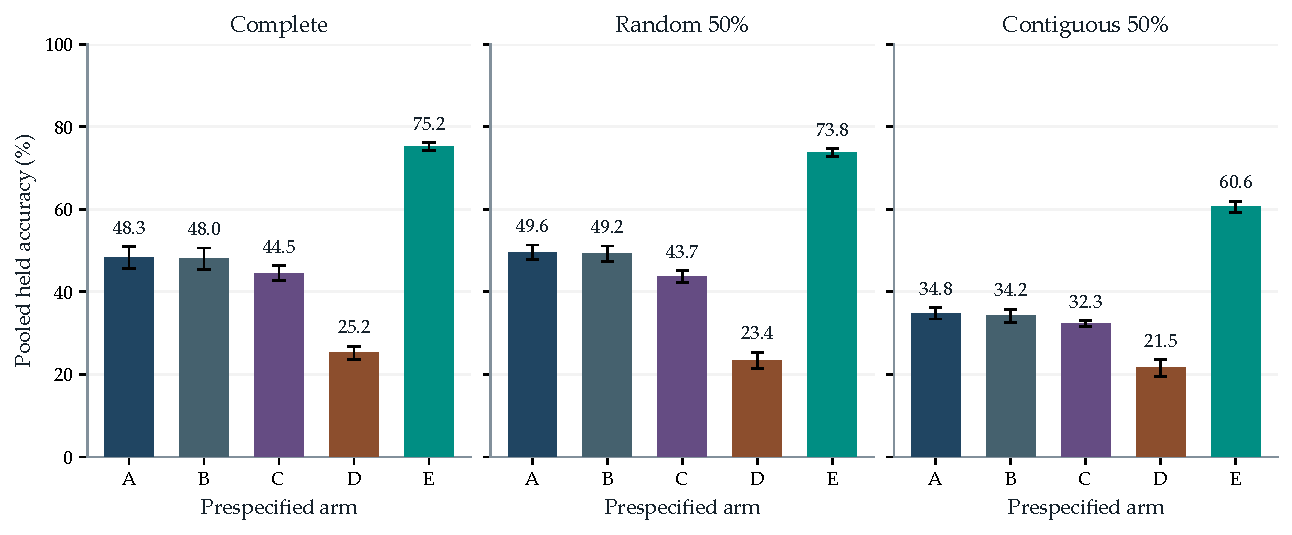
\includegraphics[width=.98\textwidth]{mira_v2_held_accuracy.pdf}
\caption{Every prespecified arm on pooled held recordings. Error bars are sample SD over five training seeds, after averaging masks within seed; they are not confidence intervals. Complete input uses one realization. Random and contiguous loss each remove 250 normalized positions shared by all channels. The feature-only arm E performs substantially better here than the hybrid arms; the plot retains the unsuccessful main candidate A and temporal control D.}
\label{fig:m2-held}
\end{figure*}
\begin{figure*}[t]
\centering
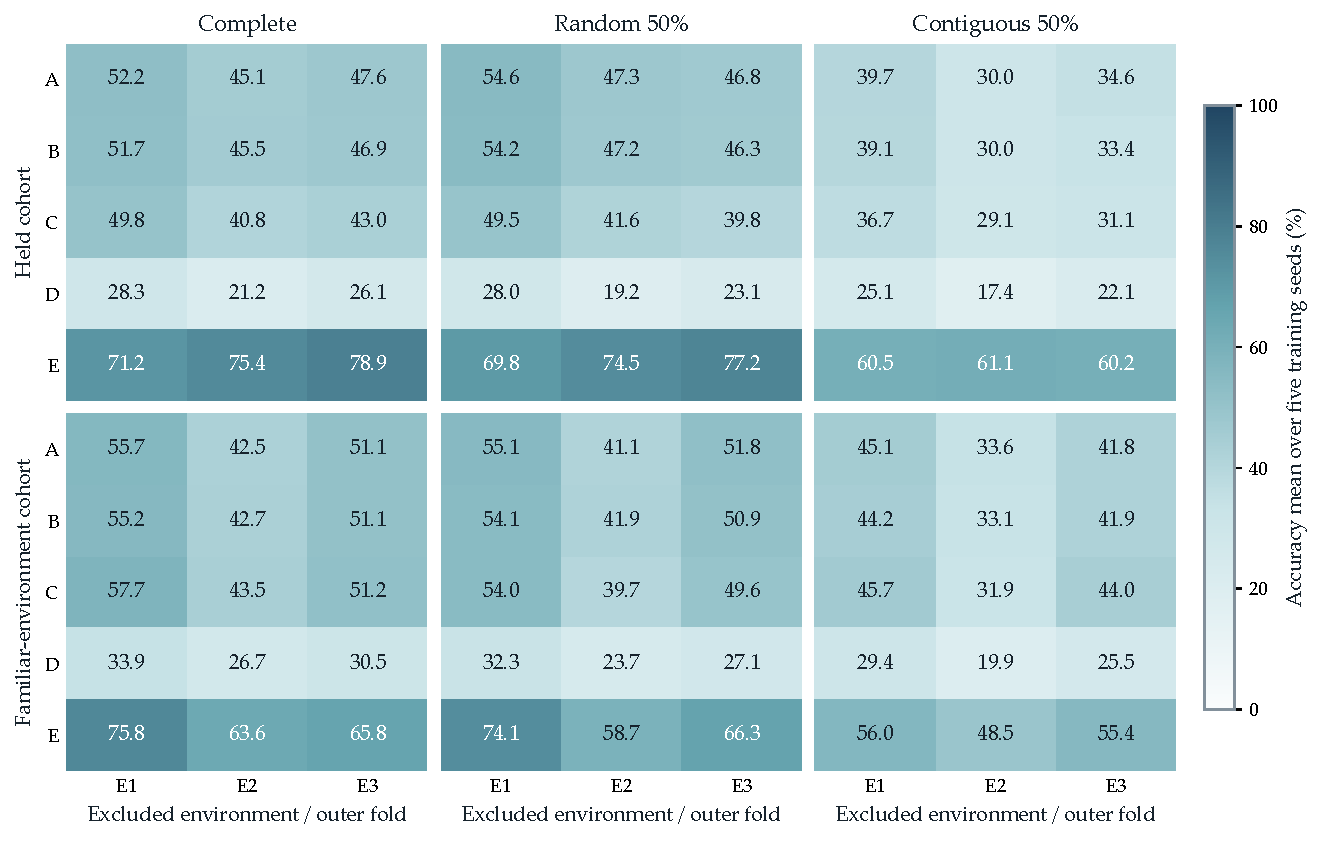
\includegraphics[width=.98\textwidth]{mira_v2_fold_domain_accuracy.pdf}
\caption{All arms, folds and cohort domains. Each cell shows mean accuracy across five training seeds after mask averaging, on a common 0--100\% colour scale. Top: the excluded environment/cohort; bottom: participants held out within the remaining two environments. E1--E3 always identify the excluded environment. Familiar and held scores are not mixed, and familiar scores are not consistently greater. Full sample SD, macro F1, NLL and Brier appear in Supplementary Tables S1--S6; Table~\ref{tab:m2-E} retains E's full 18-row breakdown in the main text.}
\label{fig:m2-folds}
\end{figure*}
\begin{figure*}[t]
\centering
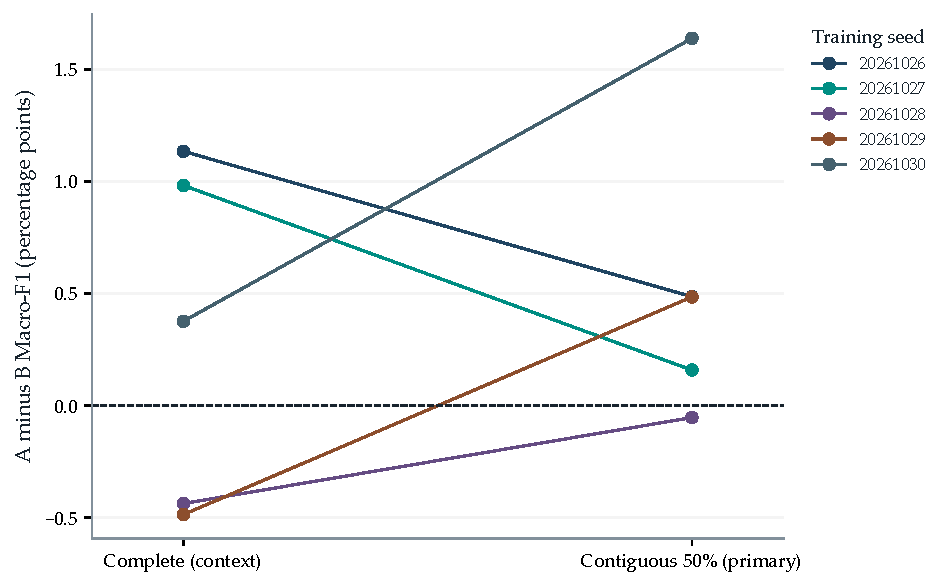
\includegraphics[width=.78\textwidth]{mira_v2_primary_paired_contrast.pdf}
\caption{Paired A minus B macro-F1 differences for each training seed. Loss-mask results are averaged before forming the five seed differences. The primary contiguous-loss contrast is $+0.543\pm0.654$ percentage points, with four positive and one negative seed difference. The clean differences are retained as context because A and B also differ on complete input. Lines join the same seed; they do not describe a physical trajectory or independent participant observations.}
\label{fig:m2-primary}
\end{figure*}


\subsection*{Interpretation, limitations and reproducibility}
The result most directly supports further investigation of a compact
fixed-feature classifier on this processed dataset. It does not validate
the original preference for the hybrid A. Since the feature-only counterpart
using B's denominator was not included, E's advantage over A--D does not
isolate support matching from the feature family, fusion, capacity or
optimization. Such a comparator and external data would require a separately
specified follow-up, not retrospective replacement of the current primary
comparison. We preserve A's weak result alongside E's encouraging result.

The source-selected MiniRocket study uses a different representation and
learning setup~\cite{dempster2021}. Its numbers and those of the present
extension do not form a controlled attribution of algorithmic superiority.
We therefore make no claim of beating MiniRocket generally, achieving
state-of-the-art performance, inventing known
covariance, masking, MLP or convolution components.

The fixed log-power floor, packet-index resampling, cell boundaries and
lags are part of the tested representation. Removing normalized positions
does not reproduce a raw timestamped acquisition outage, and observed
endpoints do not reconstruct missing movements between them. No experiment
here produces a human image, pose, temperature or vital sign, or validates
continuous live sensing. Rank truncation and padding constrain the feature-level
invariance, and the CNN has no general invariance guarantee. A possible
future source diagnostic of ranks or invalid cells must not become a
retrospective target-guided threshold search.

Input masks in the executed experiment are Boolean and the feature preparation
was checked for independence from hidden fills. A separate interface review
found that the preparation wrapper casts an externally supplied mask to
Boolean before validating it; non-binary or NaN external mask entries would
therefore be unsafe. This is a documented API precondition/limitation, not
evidence of hidden-value access in the present Boolean-mask run. The separate public prediction wrapper validates masks before conversion and rejects non-finite intermediate or output values. The archived implementation and the recorded experimental outputs remain unchanged.

The complete CPU source execution took 2,225.70 seconds; the separate
evaluation stage took 1,933.15 seconds on this machine with two compute
threads. These are execution wall times, including feature preparation and
output handling, not portable inference-latency benchmarks. Independent
source replay matched 12,600 validation probability vectors exactly; the
test-output audit checked 485,100 saved probability vectors and recomputed
1,650 per-fit/condition/domain metric rows without an additional model
forward or optimizer step. These counts include repeated views of fixed
recordings, not new samples. Five-seed summaries retain all 90
arm/fold/domain/condition combinations.

The representation cache, manifest, frozen source checkpoints, source
temperatures, saved test probabilities and report tables have SHA256 receipts.
The protocol hash begins \texttt{cc407a98f343}; the all-fit source freeze
begins \texttt{c7575d16aefd}. This audit establishes correspondence between
the declared execution and its reported numbers, not scientific priority,
absence of all implementation defects, or external validity. Because model
development followed historical target inspection and cohorts differ by
environment, a new independent dataset or prospectively untouched evaluation
is needed to assess reproducibility and generalization.
